\chapter[Formal Models]{Formal Models for Agents and Environments}
\label{cha:formal-models}

Before we begin to consider multiple agents coordinating with each
other we must first establish what we mean by an agent and how we
describe its environment. We will usually be assuming an autonoumous
agent that uses some known artificial intelligence algorithm to guide
its choice of actions. This chapter will provide a quick overview of
the agent and enviroment models used throught this book. For a more in
depth presentation we recommend \cite{russell03a}, especially
Chapters~15--17.

\section{Utility Theory}
\label{sec:utility-theory}

We commonly assume that agents are situated in a \td{state}. For
example, if the agent is a robot then its state is the state of the
world. The agent might only have a partial view of its state---a robot
might only be able to look in one direction---so the agent's current
state might not be available to the agent. Still, agents are commonly
assumed to have a \td{utility} function which gives a value to each
state. The higher the value the more the agent likes that state.

More formally, we say that the set $S$ contains all possible states
and the utility function $u_i$ for agent $i$ maps from states to real
number, that is $u_i : S \rightarrow \Re$. This utility function
defines a \td{preference ordering} for the agent over the states of
the world. 

In order to reflect real-world constraints, the utility function needs
to satisfy the following properties.

\begin{description}
\item[Reflexive] $u_i(s) \geq u_i(s)$
\item[Transitive] If $u_i(a) \geq u_i(b)$ and $u_i(b) \geq u_i(c)$ then $u_i(a) \geq u_i(c)$.
\item[Comparable] $\forall_{a,b}$ either $u_i(a) \geq u_i(b)$ or
  $u_i(b) \geq u_i(a)$.
\end{description}

We can use utility functions to describe the behavior of almost every
agent, especially selfish agents. Utilities functions are also useful
for capturing the various tradeoffs that an agent must make, along
with the value or expected value of its actions. For example, we can
say that a robot receives a certain payment (which we translate into a
utility) for delivering a package but also incurs a cost in terms of
the electricity used (which we translate into a utility) and the wear
an tear of the robot (which we translate into a utility), as well as
the opportunity cost of missing other opportunities for revenue (which
we translate into a utility). As you can see, the utility provides a
common currency for describing the various gains and losses.

Specifically, agents act so as to maximize their \td{expected utility}
which is defined as
\begin{equation}
  \label{eq:1}
  E[u(a|s)] = \sum_i P(Result_i(a)\,|\,Do(a),s) \cdot u(Result_i(a)),
\end{equation}
where $a$ is one of the agent's actions, $s$ is a state, and
$Result_i(a)$ gives us the state that results as a consequence of the
agent taken action $a$. That is, the utility that the agent can expect
if it takes action $a$ in state $s$ is the sum of utilities that the
agent receives for every state that might result from taking action
$a$ weighted by the probability of that result. 

For example, say you are given a choice between two buttons to press.
If you press button $a$ it will give you \$10 with .5 probability and
\$0 otherwise. You can calculate that the expected utility from
pressing $a$ is $.5\cdot10 + .5\cdot0 = 5$. Meanwhile, pressing button
$b$ gives you \$20 with .2 probability and \$1 otherwise which means
that pressing $b$ as an expected utility of $.2\cdot20 + .8\cdot1 =
4.8$. As such, you should press $a$ for it has the highest expected
utility.

We use the word \td{selfish} to refer to a rational agent that wants
to maximize its utility. A selfish agent only cares about its own
utility regardless of what utility the others receive. Specifically, a
selfish agent does not want to lower or increase the other agents'
utilities. Note that this definition is slightly different from the
everyday usage of the word which often implies a desire to harm other
agents. We will also often refer to selfish agents as \td{rational}
agents.

\mc{Selfish, adj. Devoid of consideration for the selfishness of
  others. ---The Devil's Dictionary}

\subsection{Utility is not Money}
\label{sec:utility-not-money}

While we will often use money and utility interchangeably we note that
research has shown that people do not have a linear utility of money.
Specifically, large amounts of money, certain lotteries, and the
amount of money the person already has all influence a person's
utility of money. Some of these effects might be due to the way we use
and spend money while others might be due to our irrationality---the
fact that most of us are really bad at math, especially probability.

For example, ay Bill has \$100M while Tim has \$0 in the bank. Someone
comes along with \$1M for one of them. Clearly, the extra million
dollars will drastically change Tim's life while Bill's life will
probably change only slightly. As such, the marginal gain in utility
for Tim is much larger for the same million dollars than it is for
Bill. Since, we assume, Bill and Tim are interchangeable (they could
be the same person at different times in his life) then we must
conclude that the utility of \$1M depends on how much money the person
already has.

Experiments have shown that people's utility function for money is
roughly logarithmic. You can determine your own curve by asking
yourself: which one would you rather have, $x$ dollars, or a $50/50$
chance at winning $2\cdot x$ dollars? Both choices are equivalent, so
we should not care either way, but for a big enough $x$ most of us
would choose the sure thing. Would you rather have \$1M or a $50/50$
chance at winning \$2M? 

Another problem is the lottery effect. People buy lottery tickets even
when they know that they are an expected loss. A typical lottery \$1
ticket is a 1 in a 10 million chance of winning \$1M. 

Recent results in behavioral economics have shown that the true
utility function is even more complicated than a simple logarithm. One
experiment shows that people are less likely to take a gamble where
the words ``lose money'' are used than one where they are not, even if
both gambles have the same expected value. The experiment is: which
option would you prefer (a) I give you \$10,000 and a 50/50 chance at
winning another \$10,000, or (b) I give you \$20,000 and then flip a
coin and if it comes out heads you have to give me \$10,000. Both of
these are equivalent but a large majority of people prefer (a).

The fact that people are not entirely rational when making choices
about money becomes important to us when we start to think about
building agents that will buy/sell/negotiate for humans. It is likely
that people will demand that agents behave the same way they would
have. That is, if a person thinks that an agent made a ``stupid
decision'' (even it was rational), he will not use that agent again.

Another example of human irrationality arises in negotiation (see
Chapter [?]), where people are sometimes more concerned with the idea
of fairness than with maximizing their utility.

\section{Markov Models}
\label{sec:markov-models}


\section{Agents}
\begin{SCfigure}
  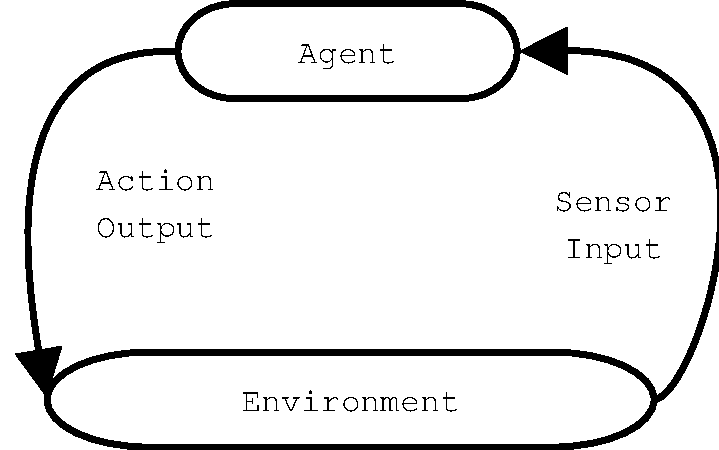
\includegraphics[width=\textwidth]{formalmodels/agent}
  \caption{Agent model.}
  \label{fig:agentmodel}
\end{SCfigure}

\begin{itemize}
\item ``An \td{agent} is a computer system that is situated in
  some environment, and that is capable of \emph{autonomous action} in
  this environment in order to meet its design objectives.''
  
\item Usually the agent only has partial control--actions
  might not have expected consequences.
  
\item Control systems.
  
\item Software demons. 
\end{itemize}

\subsection{Environment}
\label{sec:environment}

\begin{itemize}
\item \textbf{Accessible vs. inaccessible}- can the agent
  ``see'' everything? 
  
\item \textbf{Deterministic vs. non-deterministic}- do actions
  have guaranteed effect? 
  
  \item \textbf{Static vs. dynamic}- does the environment change on
    its own? 
    
  \item \textbf{Discrete vs continuous}- is the number of actions and
    percepts finite? (Does it matter?) 
  \end{itemize}

  \begin{itemize}
  \item Robotic environments are almost always
    inaccessible. Market systems are accessible, if we ignore the
    other agents' mental states. 
    
  \item Many environments are deterministic but they are complex
    enough that it does not matter. 
    
  \item Static environments are easier to deal with. Unfortunately,
    if there are other agents then they are likely changing the
    environment. 
    
  \item In the end, perceptions and actions are turned into finite
    binary numbers, so everything is approximated by discrete
    math. 
  \end{itemize}

\subsection{Agent Types}
\label{sec:agent-types}

The definitions will be used throughout the class.

  \begin{itemize}
  \item \textbf{Reactivity}- respond in a timely fashion when
    needed.
    
  \item \textbf{Pro-activeness}- satisfy internal goals. Take actions
    when it seems like they will be useful. 

  \item \textbf{Social ability}- interact with other agents in order
    to satisfy goals. 
    
  \item Pro-activeness and reactivity are often hard to
    trade-off. 
    
  \item Social ability is exceptionally hard to implement. It
    requires both sides to cooperate. 
    
  \item Agents in MASs are not intelligent in the general sense. They
    have simple specialized decision-making capabilities.
  \end{itemize}

  \begin{itemize}
  \item We can and do use objects to implement agents, but they are different.
    
  \item Agents have reactive, proactive, and social behavior. 
    
  \item Agents have their own thread of control. 
  \end{itemize}

  How to Tell: Objects do it for free; agents do it for money.


\subsection{Architectures}
\label{sec:architectures}

We now introduce some formal notation which captures the problem
domain as we have described it. We will refer to this notation and the
assumptions it implies throughout the class.

\begin{itemize}
  \item Environment $E$ changes over time ${e, e', \ldots}$. 
    
  \item An agent $Ag$ has a set of possible actions $Ac = {\alpha, \alpha', \ldots}$ 
    
  \item A run $r$ is a sequence of environmental states and
    actions $e_0 \rightarrow{\alpha_0} e_1 \rightarrow{\alpha_1} e_2
    \ldots$
    
  \item $R$ the set of all such possible runs. 
    
  \item $R^{A_c}$ be the subset of these
    that end with an action.
    
  \item $R^E$ be the subset that ends with an
    environment state.  
    
  \item $\tau: R^{A_c} \rightarrow 2^{E}$ is the
    \textbf{state transformer} function which represents the effect of
    agents' actions.
    
  \item An $Env$ is a triple $(E, e_0, \tau)$. 
\end{itemize}
    
This means that agents can take any action from $Ac$. An agents
action can change the environment, thereby leading to a new
environment. A succession of these actions and their respective new
environments is called a run. And the $\tau$ function tells us which
new environments is reached given the actions taken by all the agents. 

Note that this is a discrete synchronous model. As such, it is easy to
understand and implement but might not correctly represent the
real-time constraints of some domains.

Given this discrete environment, the agent model describes at its most
abstract how an agent might be implemented

  \begin{itemize}
  \item An agent is $Ag : R^E \rightarrow Ac$. 
    
  \item Agents are functions that map from the history of the
    environment to an action. 
    
  \item Agents are assumed to be deterministic. 
    
  \item A \textbf{system} is a pair of an $Ag$ and an $Env$. 
    
  \item The set of possible runs in a system is $R(Ag, Env)$. 
    
  \item So the sequence $(e_0, \alpha_0, e_1, \alpha_1, \ldots)$ is a
    run of $Ag$ in $Env = (E, e_0, \tau$).
    
  \item Two agents are said to be \textbf{behaviorally equivalent} wrt
    $Env$ iff $R(Ag1, Env) = R(Ag2, Env)$.
  \end{itemize}

Most agent implementations, however, are not deterministic. Even the
simplest of agents incorporates some adaptability while more
sophisticated agents implement full machine learning algorithms. This
fact limits the usefulness of this formalism. We can extend the
formalism by letting $Ag$ vary with time. That is, let $Ag^t$
represent the agent's function at time $t$. We would then need to
specify how $Ag^{t+1}$ is related to $Ag^t$, that is, how an agent's
\emph{entire} behavior at time $t+1$ is related to its behavior at
time $t$. This is not easy task. It remains an open problem.


  \begin{itemize}
  \item We can now formally define a reactive agent as $Ag: E
    \rightarrow Ac$.

  \item Notice that it only considers one environmental state--the latest one. 

  \item They can implement fewer behaviors than the standard agent. 
  \end{itemize}

Reactive agents are very useful since they do not require state. We
will be re-visiting this idea throughout the course.


\begin{SCfigure}
  \centering
  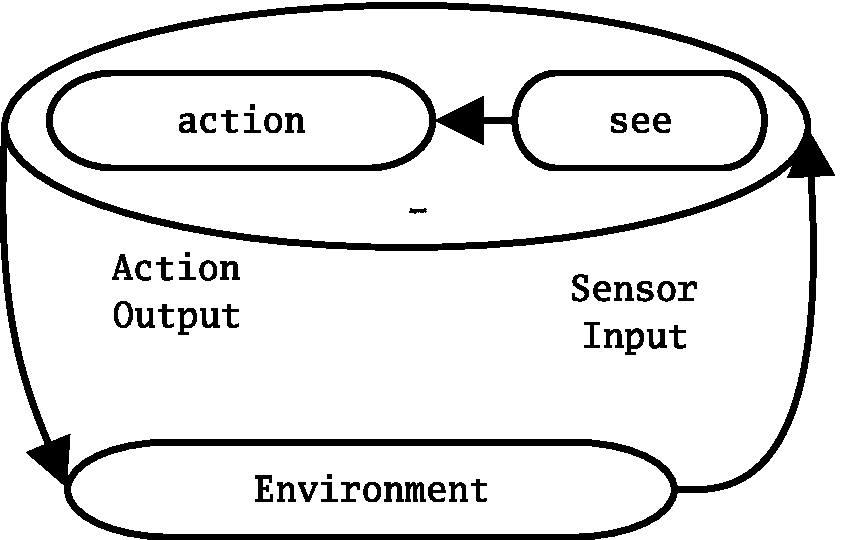
\includegraphics[width=\textwidth]{formalmodels/perception}
  \caption{Perception}
  \label{fig:perception}
\end{SCfigure}
\begin{itemize}
\item Usually the environment can have a very large number of
  states and the agent's perceptions can only capture part
  (inaccessible). 
  
\item We define \textbf{see}: $E \rightarrow Per$. Where $Per$ is the set
  of percepts. 
  
\item We define \textbf{action}: $Per^{*} \rightarrow Ac$.
  
\item What if $e$ and $e'$ get mapped to the same $Per$? 
  
\end{itemize}

Devising a good \textbf{see} function is known as the ``mapping
problem'' in machine learning. This is the problem of how to reduce a
nearly infinite set of possible inputs into a large but manageable set
of inputs which are then fed into the machine learning algorithm. We
want to throw away irrelevant information. For example, if the goal is
to recognize faces by looking at pictures we might throw away all
color information as well as the parts of the picture that are not the
face. Unfortunately implementing these functions correctly is
usually impossible and, in the end, we often end up circling back to
the original problem: how do we recognize a face? Still, in most
situations there are always a few obvious bits of information that are
easy to throw and do not affect performance.

If the agent remembers parts of its perception then we can say that
the agent has a state.

    \begin{SCfigure}
      \centering
      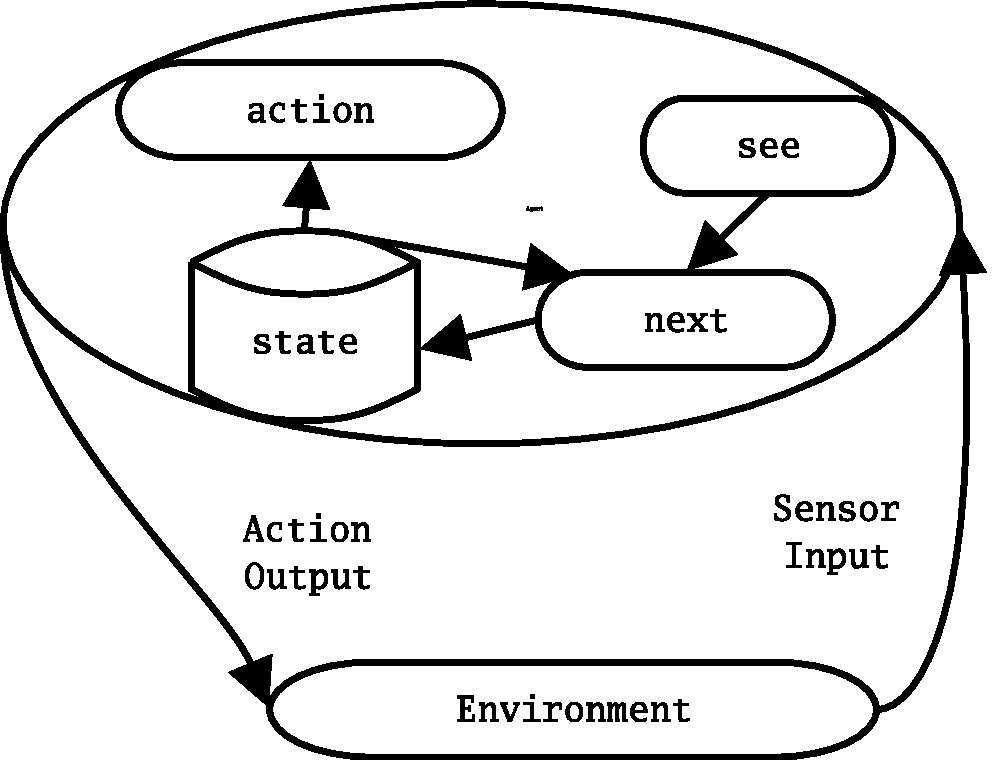
\includegraphics[width=\textwidth]{formalmodels/state}
      \caption{State}
      \label{fig:state}
    \end{SCfigure}

    \begin{itemize}
    \item Agents can maintain an internal state $I$ and use it when
      determining what action to take.
      
    \item \textbf{see}: $E \rightarrow Per$. 
      
    \item \textbf{action}: $I \rightarrow Ac$
      
    \item \textbf{next}:$I \times Per \rightarrow I$
      
    \item They have the same expressive power as standard agents, but they are easier to implement. 
    \end{itemize}

Note that many variations on this model are possible. For example, the
agent could take an action based on the state and perception, or the
new state could be determined by the current state and the actions of
the other agents. However, all these cases share the common fact that
the agent maintains a local state: it remembers something about its
past. Since memory is cheap, we can easily build agents that remember
a lot but it is much harder to build agents that use these memories
effectively.


%%% Local Variables: 
%%% mode: latex
%%% TeX-command-default: "PDFlatex"
%%% TeX-master: "~/wp/mas/mas"
%%% End: 
